\begin{figure}
\centering
\begin{subfigure}{80mm}
  \centering
    \includegraphics[width=80mm]{triangleplot_CUZNS298.png}
    \caption{Cu, Zn, S Ternary Diagram}
    \label{fig:CuZnS}
\end{subfigure}%
\begin{subfigure}{80mm}
 \centering
    \includegraphics[width=80mm]{triangleplot_CUZNSN298.png}
    \caption{Cu, Zn, Sn Ternary Diagram}
    \label{fig:CuZnSn}
\end{subfigure}
\begin{subfigure}{80mm}
 \centering
    \includegraphics[width=80mm]{triangleplot_CUSNS298.png}
    \caption{Cu, Sn, S Ternary Diagram}
    \label{fig:CuSnS}
\end{subfigure}
\caption{Ternary Diagrams of the remaining face, post 'Tie-line' calculations.}
\label{fig:RemainingFaces}
\end{figure}

In Figures 1 and 3, we see completed Ternary Phase Diagrams for the four faces of the original quaternary diagram - with all crossing points removed and the stable pahses of the diagrams present.
These allow us to further produce a Quaternary diagram with indicative 'tie-phases', and as such locate the thermodynamic area we are most likely to find CZTS in. An example of one of the possible candidate 'tie-phases' is presented in figure 2. This and four other candidate 'tie-phases' were examined to find a 'tie-phase' with the correct 2:1 ratio of sulphur to the other elements present within CZTS. Through determination of the ratios, I found only one acceptable candidate: $ZnS$, $Sns_2$, $Cu_2S$, though another would fit the general ratio, that of $ZnS$, $Sn_2s_3$, $Cu_2S$ however, this did not have the correct ratio of Copper, Zinc and Tin and as such was dismissed.

Presented in figure 4 is a diagram demonstrating the theoretical area where CZTS is most likely to occur; also presented are the areas which are generally either more "rich" or "poor" in on of the elements. This fits with the work presented by Olekseyuk in 2004.\citep{olekseyuk_phase_2004}

\begin{figure}
\centering
 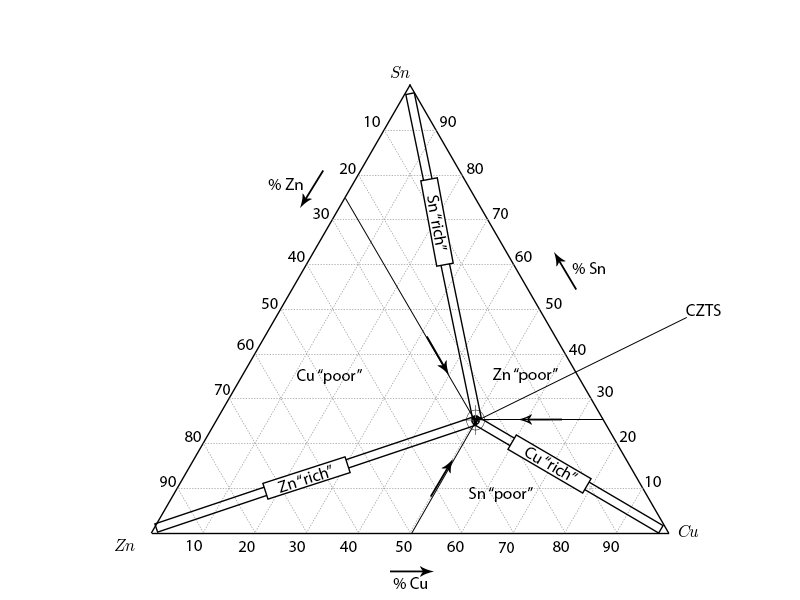
\includegraphics[width=80mm]{ZnSSn2S3Cu2S-general}
    \caption{Location of CZTS, and labelled secondary phases.}
    \label{fig:ZnSSn2S3Cu2S}
\end{figure}
